% !TeX program = xelatex
% !TeX encoding = UTF-8
\documentclass[12pt,letterpaper,oneside]{report}

% ===== 字体（请使用 XeLaTeX 编译） =====
\usepackage{fontspec}
\defaultfontfeatures{Ligatures=TeX}

% ===== 页面与排版 =====
\usepackage[letterpaper,margin=1in,headheight=15pt]{geometry}
\usepackage{setspace}
\onehalfspacing
\usepackage{microtype}
\usepackage{indentfirst}
\setlength{\parindent}{2em}
\setlength{\parskip}{0.25em}

% ===== 数学、单位、表格与图片 =====
\usepackage{amsmath,amssymb,mathtools}
\usepackage{graphicx}
\graphicspath{{figures/}}
\usepackage{booktabs}
\usepackage{array}
\usepackage{caption}
\usepackage{subcaption}
\usepackage{enumitem}

% ===== 颜色 =====
\usepackage{xcolor}
\definecolor{UMblue}{HTML}{00274C}
\definecolor{UMmaize}{HTML}{FFCB05}

% ===== 文献 =====
\usepackage[round,authoryear]{natbib}

% ===== PDF 链接、书签与导航 =====
% hyperref 应尽量靠后加载；cleveref 必须在 hyperref 之后。
\usepackage{hyperref}
\usepackage{bookmark}
\usepackage[nameinlink,noabbrev]{cleveref}
\hypersetup{
  unicode=true,
  colorlinks=true,
  linkcolor=UMblue,
  citecolor=UMblue,
  urlcolor=UMblue,
  linktoc=all,
  bookmarksopen=true,
  bookmarksnumbered=true,
  pdfstartview=FitH
}

% ===== 页眉页脚 =====
\usepackage{fancyhdr}
\usepackage{lastpage}

\newcommand{\ContentsLink}{%
  \hyperlink{toc}{\textcolor{UMblue}{\bfseries Back to Contents}}%
}

\newcommand{\PageNavigation}{%
  \Acrobatmenu{PrevPage}{\textcolor{UMblue}{Previous}}%
  \quad\textcolor{gray}{|}\quad
  \hyperlink{toc}{\textcolor{UMblue}{Contents}}%
  \quad\textcolor{gray}{|}\quad
  \textcolor{black}{\thepage/\pageref*{LastPage}}%
  \quad\textcolor{gray}{|}\quad
  \Acrobatmenu{NextPage}{\textcolor{UMblue}{Next}}%
}

\fancypagestyle{reportstyle}{
  \fancyhf{}
  \fancyhead[L]{\small\nouppercase{\leftmark}}
  \fancyhead[R]{\small\ContentsLink}
  \fancyfoot[C]{\small\PageNavigation}
  \renewcommand{\headrulewidth}{0.4pt}
  \renewcommand{\footrulewidth}{0.4pt}
}

% chapter 首页默认使用 plain；重定义后仍保留全部导航。
\fancypagestyle{plain}{
  \fancyhf{}
  \fancyhead[L]{\small\nouppercase{\leftmark}}
  \fancyhead[R]{\small\ContentsLink}
  \fancyfoot[C]{\small\PageNavigation}
  \renewcommand{\headrulewidth}{0.4pt}
  \renewcommand{\footrulewidth}{0.4pt}
}

% ===== 目录深度与编号深度 =====
\setcounter{tocdepth}{2}    % 目录显示到 subsection
\setcounter{secnumdepth}{3} % 正文编号到 subsubsection

% ===== 常用命令示例 =====
\newcommand{\vect}[1]{\boldsymbol{#1}}
\newcommand{\dd}{\mathop{}\!\mathrm{d}}


\newcommand{\ReportTitle}{Lateral Dynamics and Control of a Unicycle Robot}
\newcommand{\ReportSubtitle}{Report after implementing the linear motor}
\newcommand{\ReportAuthor}{Gao Shenghan}
\newcommand{\ReportInstitution}{University of Michigan}
\newcommand{\ReportDepartment}{Department of Mechanical Engineering}
\newcommand{\ReportCourse}{Course / Project Name}
\newcommand{\ReportAdvisor}{Advisor: Prof. Name}
\newcommand{\ReportDate}{\today}

\hypersetup{
  pdftitle={\ReportTitle},
  pdfauthor={\ReportAuthor},
  pdfsubject={\ReportCourse},
  pdfkeywords={report, LaTeX}
}

\begin{document}
\pagestyle{reportstyle}
\pagenumbering{arabic}
\setcounter{page}{1}

\thispagestyle{reportstyle}
\begin{center}
  \vspace*{2.0cm}

  {\Huge\bfseries \ReportTitle\par}
  \vspace{0.5cm}
  {\Large \ReportSubtitle\par}

  \vfill

  \begin{tabular}{rl}
    Author:      & \ReportAuthor \\
    Date:        & \ReportDate
  \end{tabular}

  \vfill
  \hyperlink{toc}{\colorbox{UMmaize}{\textcolor{UMblue}{\bfseries\strut Go to Contents}}}
  \vspace{1.0cm}
\end{center}
\clearpage

% \include{chapters/00-abstract}

\clearpage
\phantomsection
\hypertarget{toc}{}
\tableofcontents

% \clearpage
% \listoffigures
% \clearpage
% \listoftables

\include{chapters/01-introduction}
\chapter{Theoretical Analysis and Simulation}
\label{chap:theory-simulation}

This chapter presents the theoretical analysis and numerical simulation of the lateral dynamics of the unicycle robot. The purpose of this analysis is to evaluate the feasibility of the proposed balancing method and controller design before conducting experiments on the physical system.

\section{Modeling of the Lateral Dynamics}

\subsection{Reduced Lateral-Dynamics Model}

The complete unicycle robot contains strongly coupled longitudinal and lateral motions, as illustrated in Figure~\ref{fig:fullnotation}. Developing and analyzing a full model that includes all of these motions is complicated. Therefore, in this chapter, the longitudinal and lateral dynamics are assumed to be approximately decoupled, allowing the lateral motion to be studied independently.

\begin{figure}[htbp]
  \centering
  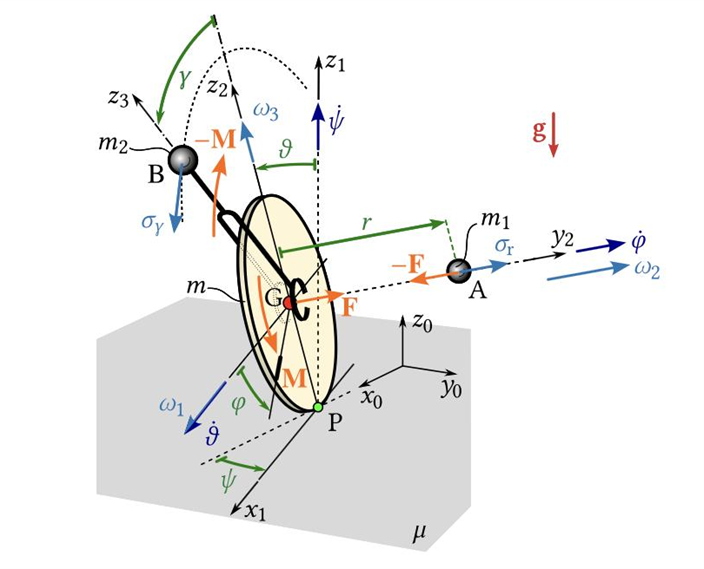
\includegraphics[width=0.75\textwidth]{02/fullnotation.png}
  \caption{Full mechanical model and notation of the unicycle robot.}
  \label{fig:fullnotation}
\end{figure}

The resulting reduced model of the lateral dynamics is shown in Figure~\ref{fig:partialmodel}. The reduced model is described using the generalized coordinates

\begin{equation}
q_1=\theta,
\qquad
q_2=r-R\theta,
\label{eq:generalized-coordinates}
\end{equation}

where $q_1$ is the lateral lean angle and $q_2$ is the rod position relative to the lateral motion of the wheel center. The corresponding generalized velocities are

\begin{equation}
u_1=\dot{q}_1=\dot{\theta},
\qquad
u_2=\dot{q}_2=\dot{r}-R\dot{\theta}.
\label{eq:generalized-velocities}
\end{equation}

Therefore, the physical rod position and velocity can be recovered from

\begin{equation}
r=q_2+Rq_1,
\qquad
\dot{r}=u_2+Ru_1.
\label{eq:rod-position-recovery}
\end{equation}

To simplify the notation, the constant rotational inertia is defined as

\begin{equation}
J
=
m_wR^2
+
m_b(R+h)^2
+
I_w
+
I_b
+
I_{\mathrm{rod}},
\label{eq:constant-J}
\end{equation}

and the combined gravitational coefficient is defined as

\begin{equation}
G
=
m_wgR
+
m_bg(R+h).
\label{eq:constant-G}
\end{equation}

Here, $m_b$ is the battery mass, which is modeled as the primary pendulum mass of the robot. The parameter $G$ combines the gravitational moments produced by the wheel and the battery assembly.

Using these definitions, the nonlinear lateral dynamics can be written compactly as

\begin{equation}
\begin{bmatrix}
J+m_{\mathrm{rod}}r^2 & 0 \\
0 & m_{\mathrm{rod}}
\end{bmatrix}
\begin{bmatrix}
\dot{u}_1 \\
\dot{u}_2
\end{bmatrix}
=
\begin{bmatrix}
FR
-m_{\mathrm{rod}}gr\cos\theta
+G\sin\theta
-m_{\mathrm{rod}}r
\left(
2u_1u_2+Ru_1^2
\right)
\\[6pt]
F
-m_{\mathrm{rod}}g\sin\theta
+m_{\mathrm{rod}}ru_1^2
\end{bmatrix}.
\label{eq:simplified-lateral-model}
\end{equation}

The four-dimensional state vector is defined as

\begin{equation}
\mathbf{x}
=
\begin{bmatrix}
x_1 \\
x_2 \\
x_3 \\
x_4
\end{bmatrix}
=
\begin{bmatrix}
q_1 \\
q_2 \\
u_1 \\
u_2
\end{bmatrix}
=
\begin{bmatrix}
\theta \\
r-R\theta \\
\dot{\theta} \\
\dot{r}-R\dot{\theta}
\end{bmatrix}.
\label{eq:lateral-state-vector}
\end{equation}

In terms of the state variables, the physical rod position is

\begin{equation}
r=x_2+Rx_1.
\label{eq:rod-position-state}
\end{equation}

The complete four-dimensional model can then be written in the following compact implicit first-order form:

\begin{equation}
\begin{bmatrix}
1 & 0 & 0 & 0 \\
0 & 1 & 0 & 0 \\
0 & 0 & J+m_{\mathrm{rod}}(x_2+Rx_1)^2 & 0 \\
0 & 0 & 0 & m_{\mathrm{rod}}
\end{bmatrix}
\begin{bmatrix}
\dot{x}_1 \\
\dot{x}_2 \\
\dot{x}_3 \\
\dot{x}_4
\end{bmatrix}
=
\begin{bmatrix}
x_3
\\[4pt]
x_4
\\[4pt]
FR
-m_{\mathrm{rod}}g(x_2+Rx_1)\cos x_1
+G\sin x_1 \\
-m_{\mathrm{rod}}(x_2+Rx_1)
\left(
2x_3x_4+Rx_3^2
\right)
\\[6pt]
F
-m_{\mathrm{rod}}g\sin x_1
+m_{\mathrm{rod}}(x_2+Rx_1)x_3^2
\end{bmatrix}.
\label{eq:four-dimensional-lateral-model}
\end{equation}

Equation~\eqref{eq:four-dimensional-lateral-model} is used as the nonlinear plant model for the controller design and numerical simulations presented in the following sections.
\chapter{Results and Discussion}
\label{chap:results}

\section{Results}

Tables should have captions above them, as in \cref{tab:sample}.

\begin{table}[htbp]
  \centering
  \caption{Example results table.}
  \label{tab:sample}
  \begin{tabular}{lrr}
    \toprule
    {Case} & {Value} & {Error (\%)} \\
    \midrule
    Baseline & 1.00 & 0.0 \\
    Test A   & 1.12 & 12.0 \\
    Test B   & 0.94 & 6.0 \\
    \bottomrule
  \end{tabular}
\end{table}

\section{Discussion}

Interpret the results rather than repeating them. Explain the mechanism,
compare the observations with expectations, and state the limitations.

\subsection{Uncertainty and Limitations}

Record measurement uncertainty, modeling assumptions, and conditions under
which the conclusion may not hold.

\chapter{Conclusion}
\label{chap:conclusion}

Summarize the main finding, its significance, and the most useful next step.
Do not introduce new results in this chapter.

\section{Future Work}

List specific improvements or experiments that follow directly from the
limitations identified in \cref{chap:results}.


\clearpage
\phantomsection
\addcontentsline{toc}{chapter}{References}
\bibliographystyle{plainnat}
\bibliography{references}

% \appendix
% \chapter{Supplementary Derivation}
\label{app:derivation}

Place long derivations, additional figures, code excerpts, or calibration data
in appendices. Appendix chapters are lettered automatically.


\end{document}
